\section{Shading}

\subsection{Direct Illumination}
Direct illumination is the radiance contribution at a surface directly from the light sources in the scene, in path notation
this is \textbf{LDE} this term is responsible for the majority of detail in the scene, as a result we use raytracing to calcualte
the radiance from direct illumination, it is possible to calculate the radiance due to this term from the photon map but this
approach leads to noise in the final image even when using a high number of photons in the radiance estimate, a comparison of
direct illumination with raytraceing and the photon map can be seen in Figure~\ref{fig:direct_compare}

\todo{Add}
\missingfigure{Direct raytraced and photon mapped compare}
\begin{figure}
\label{fig:direct_compare}
\end{figure}

\subsubsection{Texture Mapping}
Performing texture mapping requires the ability to query the texture coordinates at a point of intersection, for mesh objects this
will interpolate the barycentric coordinates for the triangle of intersection, spheres use a spherical mapping that uses the
spherical coordinates to generate u,v values.

\subsection{Specular Reflection and Transmission}
\subsubsection{Schlick Approximation}
Transmissive surfaces reflect a proportion of the radiance incident at the surface as it passes from a material with a different
index of refraction, this proportion is determined by the fresnell equation for dielectrics, which is a function of the refractive
index of the two materials and the incident angle, this is given by equation ~\ref{eq:fresnel}, this is unfortuanattly an expensive
calculation, an approximation by Schlick \todo{cite} reduces the computational nessaccarry, this is given in Equation~\ref{eq:schlick}


\missingfigure{Non, proper and schlick reflection}

\begin{equation}
\cos{\theta_t} = \sqrt{1 - \left(\frac{\eta_1}{\eta_2}\sin{\theta_i}\right)^2}
\end{equation}

\begin{equation}
R_f(\theta)
=
\frac{
	\left(
	\frac
	{
	\eta_2 \cos{\theta_i} - \eta_1 \cos{\theta_t}
	}
	{
	\eta_2 \cos{\theta_i} + \eta_1 \cos{\theta_t}
	}
	+
	\frac
	{
	\eta_1 \cos{\theta_i} - \eta_2 \cos{\theta_t}
	}
	{
	\eta_1 \cos{\theta_i} + \eta_2 \cos{\theta_t}
	}
\right)^2
}{2}
\label{eq:fresnel}
\end{equation}

\begin{equation}
R_s(\theta)=R_0 + \left(1 + R_0\right)\left(1 - \cos\theta\right)^5
\label{eq:schlick}
\end{equation}

As with other aspects of the system where multiple rays can be spawned from a surface interaction (in this case one reflected and one refracted ray)
we use russian roulette in order to determine if we reflect or refract.

\subsection{Nearest Neighbour Search}
\todo{psuedocode}

\subsection{Diffuse Interreflection}
While it is possible to estimate the contribition to the radiance at an intersection point directly from the photon map this
approach can cause visual artifacts due to variance in the estimate in order to reduce these artifacts we perfom a final gather
stage at the point of intersect that produces a diffuse ray that is traced into the scene until a non-specular object is intesected,
we then perform the radiance at this point and use this information to estimate the radiance incident at the original point of intersection.
In order for the final gather to produce a correct estimate of the radiance we need to perform this stage multiple times per pixel, as we
are performing distributed raytracing this is a trivial addition. When calcualting the radiance for the final gather it has been shown \todo{cite}
that if the distance of the final gather point is lower than some threshold perfoming an additional diffuse bounce reduces errors at geometry
such as sharp corners where the radiance estimate can be inaccurate due to accounting for photons not truly at the surface.

\begin{figure}
\centering
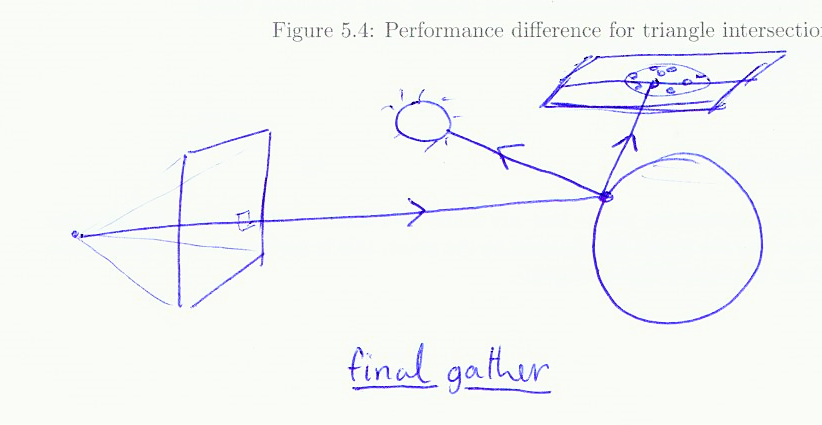
\includegraphics[width=\textwidth]{./images/final_gather.png}
\label{fig:final_gather}
\caption{Final Gather}
\end{figure}

\subsection{Caustics}
Caustics are generated from the focusing of light by specular transmission, an example of this would be light focused by a magnifying glass or
light rings at the bottom of a cup. As we have explicitly stored the specular paths we can evaluate the contribution to the radiance by
using the photon map radiance estimate at the intersection point.
\todo{Possibly add importance sampling}
